\subsection{RavenClaw: Dialog Management Using Hierarchical Task Decomposition and an Expectation Agenda \cite{Bohus2003}}

This paper describes \emph{RavenClaw}, a new dialog management framework used in the \emph{CMU Communicator}. RavenClaw introduces a clear separation between task and discourse behaviour specification, and allows rapid development of dialog management components for spoken dialog systems operating in complex, goal-oriented domains.

Dialog management maintains continuity over turns in a conversation between human and computer. The authors believe that the essence of dialog management resides in performing two functions: interpreting user inputs with respect to tasks within the domain, and maintaining the coherence over time. Based on this philosophy, the proposed RavenClaw is a two-tier architecture (cf. Figure \ref{fig:raven_arch}). The \emph{Dialog Task Specification} layer captures all the domain-specific dialog logic. The \emph{Dialog Engine} is a domain-independent component that controls the dialog and contributes basic conversational strategies (e.g., timing and turn-taking behaviour, grounding behaviour, etc.).

\begin{figure}[h]
  \centering
  % Requires \usepackage{graphicx}
  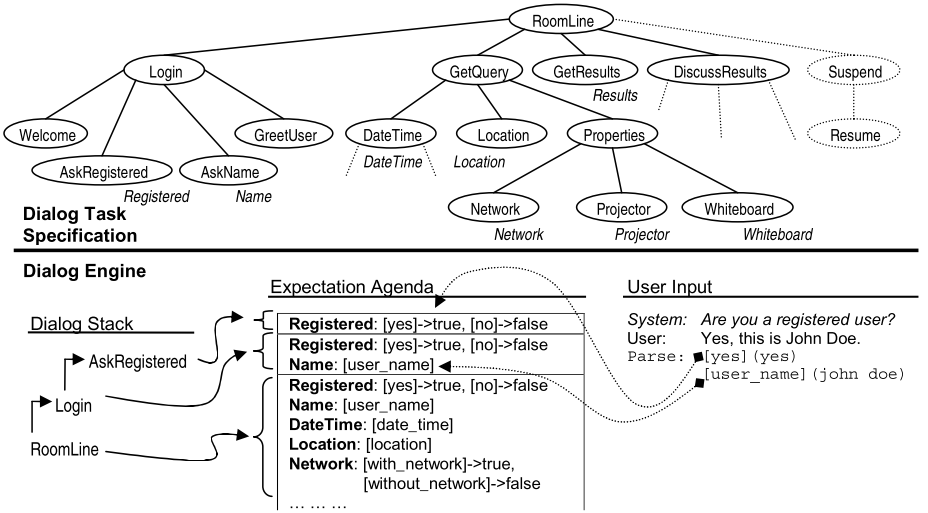
\includegraphics[width=\linewidth]{ravenclaw_arch.png}\\
  \caption{RavenClaw architecture.}\label{fig:raven_arch}
\end{figure}

The domain-specific dialog control is represented in the Dialog Task Specification level using a tree of dialog agents, with each agent handling a certain part of the dialog task. The proposed architecture uses hierarchical task decompositions, which are traditionally used for task execution in robotics. Two categories of dialog agents populate the task tree: \emph{fundamental dialog agents} and \emph{dialog agencies}. The fundamental dialog agents appear as leaf nodes (e.g. \textbf{Welcome}, \textbf{AskRegistered}) and represent atomic dialog actions. The non-terminal nodes in the tree are dialog agencies (e.g. \textbf{Login}, \textbf{GetQuery}), which control the execution of their subsumed agents, capturing the higher level temporal and logical structure of the dialog task.

The Dialog Engine is the core component in RavenClaw and controls the dialog by executing the Dialog Task Specification. Dialog flow is generated by interleaving \emph{Execution Phases} and \emph{Input Phases}. In an Execution Phase, the various agents in the task tree are executed and generate the system's behaviour. In an Input Phase, the system collects and incorporates the information from the user's input.

A characteristic which greatly influences the usability and ultimately the success of spoken dialog systems is their ability to employ a rich set of conversational strategies. These encompass grounding behaviours (e.g. confirmations, disambiguations, etc.), turn-taking and timing behaviours. RavenClaw provides automatic support for all the above mentioned conversational strategies. Internally, they are implemented as dialog agencies, in the same manner as the domain-specific dialog task tree.

Finally, the paper presents five systems using RavenClaw-based dialog managers (LARRI, the Intelligent Procedure Assistant, BusLine, RoomLine and TeamTalk). These implemented systems show that the proposed framework can be easily adapted to different domains, indicating that RavenClaw is with a high degree of versatility and scalability.
